\chapter{Implementace frontendu}
Frontend byl vyvíjen jako single-page aplication pomocí javasriptu a reactu.
Navržen tak aby byl jednuduše ovladatelný přehledný a především velmi rychlý.

\section{Server}
Celá aplikace frontendu je uložena na serveru, včetně zdrojových kódů.
Uživatel si ale stahuje pouze zkompilovanou aplikaci a případné externí zdroje.
\subsection{Kompilace}
Ačkoliv je javascript scriptovací jazyk a kompilaci provádí až za běhu, tak je možné
jej zkompilovat předem. Při této kompilaci knihvny \textbf{webpack} a
\textbf{babel} provedou několik zásadních kroků, z nichž nejdůležitějsími jsou
projití kódu a jeho převedení na ECMAScript 5 (kvůli zpětné kompabilitě), přetřízení a sloučení
knihoven do jednoho zdrojového souboru (javascript se k uživateli dostane při prvním dotazu na server) a
minifikace výsldného souboru, jež dokáže inteligentně projít kód a optimalizovat jeho textovou délku,
čím výrazně sníží čas potřebný k načtení stránky. 
\subsection{NPM}
Celá aplikace má strukturu balíčku NPM (node package manager), tudíž ji lze snadno
spustit kdekoliv, kde je nainstalovaný nodejs a knihovna npm.
Zároveň udržuje pomocí souboru \textbf{package.json} přehled o potřebných knihovnách (dependencies) a
obsahuje též různé spouštěcí scripty, např. script pro buil produkční erze aplikace.

\section{Knihovny}
Aplikace se skládá z více než tisíce knihoven a modulů, tudíž se podíváme
pouze na ty nejvetší a nejdůležitější z nich.

\subsection{React}
Tato JavaScriptová knihovna je vyvinuta společností Facebook a slouží pro tvorbu uživatelského rozhraní.\\
Jejím základem je vykreslování pomocí tkz. single-page a je vhodná zejména pro aplikace, kde se často mění data.
Využívá pozměněné JavaScriptové syntaxe známe jako JSX (JavaScript XML), která umožňuje
pracovat s HTML tagy uvnitř JavaScriptového kódu, bez nutnosti práce DOM objektem.\\
Výhodou single-page aplikace je pak i optimalizovaná práce s DOM objektem, který je bottleneck
(úzkým hrdlem) při nesprávném použití (nebo lépe řečeno, při kterémkoliv použití, které něco s DOM objektem dělá).

\subsection{Material-UI}
Společnost Google (aktuálně Alphabet Inc.) se v roce 2014 rozhodla sjednotit svou grafickou podobu a
vyvynula designový jazyk, jež se stal příručkou jak vytvářet uživatelsky přívětivé aplikace (nejen na webu, ale třeba
i v aplikaci mobilním telefonu nebo tabletu). Základem tohoto stylu je realistická práce se světlem
a uživatelskou interakcí. Vše odlehčené a intuitivní. Součástí tohoto grafického jazyka jsou i
lehce čitelné fonty (Roboto), pochopitelné ikonky a systém barev a jejich kombinací.

\subsection{i18n}
Jelikož je projekt mířen i na nečeské uživatele, vyskytla se potřeba rozhranní překládat.
Jednoduchým přístupem by bylo zkompilovat několik aplikací každou pro jiný jazyk, tudíž
by se překlad odehrával na straně serveru. Bohužel to není nejoptimálnější řešení a
tudížbyla využita knihovna i18n, jež funguje na podobném principu jako single-page aplication a
to sice, že dokáže měnit překlad stránky bez nutnosti stránku přenačíst a zároveň hlavní aplikace
neobsahuje všechny jazyky při prvním načtení. Jazyky se postupně dostahují dle preference uživatele
(vše samozřejmě na pozadí bez uživatelského zásahu).\\
Velkou výhodou tohoto systému může být například situace, kdy je potřeba přeložit jeden nápis na stránce,
případně sehnat anglický ekvivalent a nechceme přenačtením stránky přijít o již vyplněná data.

\subsection{Babel}
Jak už bylo zmíněno výše, aplikace se kompiluje a za tuto část je zodpovědná právě knihovna Babel.\\
Hlavní výhodou je kompilace kódu v ES6+ (EcmaScipt v6, neboli Javascript v6) do ES5 (EcmaScipt v5, neboli Javascript v5)
Tímto převodem získáme zpětnou kompatibilitu pro starší javascriptové enginy.

\subsection{Webpack}
Aby se z tak obrovského množství knihoven a souborů stal jediný spustitelný soubor pomáhá
knihovna Webpack, která má za úkol kód zkomprimovat a sjednotit. Touto optimalizací si ušetříme
množství dotazů, jež bude muset náš server příjmout (a ekvivalentně s tím uživatel odeslat).\\
Zároveň nám umožňuje používat formát \textbf{SCSS}, což je nadstavba nad klasickým CSS, jež 
rozpoznávají prohlížeče a dovoluje nám takto vytvářet \textbf{stylovací moduly}.

\section{Rozhraní}
Jelikož se jedná o složitější systém a všechno nemůže být naházené v jediném souboru, tak 
je použita hierarchie která vypadá násldovně:
\begin{itemize}
	\item Hlavní soubor celého webu - provádí routing a obaluje celou aplikaci pomocnými wrapery
		(např. i18n překladač, Mui pro jednotný styl, SnackbarProvider
		pro vyskakovací toasty a CookiesProvider pro jednotný přístup ke cookies)
	\item Scény - Stránky diametrálních vlastností a funkcionalit
	\item Komponenty - malé na sobě nezávislé \uv{černé krabičky} poskytující určitou funkcionalitu
\end{itemize}


\subsection{Scény}
\subsubsection{Admin}
Administrační rozhranní je přístupné pouze s oprávněním \uv{execute}.
Zde může administrátor nebo správce uživatelů vytvářet nové účty nebo
konfigurovat stávající.\\
Jelikož se hesla v databázi ukládají zahešovaná, tak je nelze zobrazit ani adminovi.
Dala by se přidat funkcionalita pro jejich crackovaní, aby se nalezli uživatelé se
slabými hesly, ale to by bylo zbytečné plýtvání serverovými prostředky.
\begin{center}
	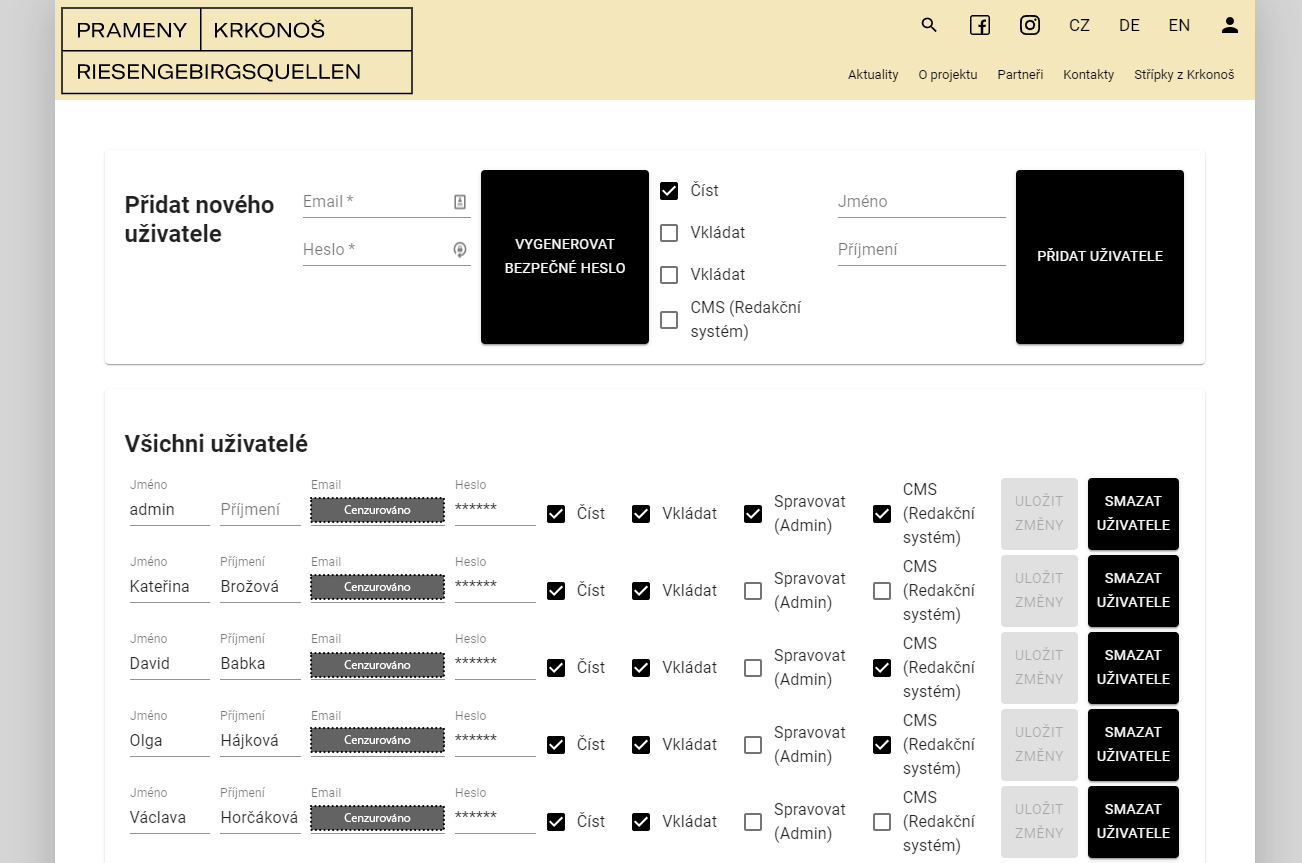
\includegraphics[width=.8\textwidth]{img/adminScene.png}
\end{center}

\subsubsection{CMS}
Vytváření a editace obsahu stránek se provádí v redakčním systému (Content Management System, zkráceně CMS).
Do něj se uživatel dostane pouze po přihlášení a s platnými právy pro redakční systém.\\
Úpravy redaktor provádí v prostředí WYSIWYG (What you se is what you get, neboli co vidíš to dostaneš).
V pravém panelu pak zadá název, případně krátký popis, který se hodí např. pro aktuality a kategorii.\\
WYSIWYG editro podporuje velkou škálu stylování a formátování. Velkou výhodou je možnost nahrávání obrázků,
kdy se po přetažení automaticky uloží na server do složky uploads a jejich odkaz se vloží do stránky.
\begin{center}
	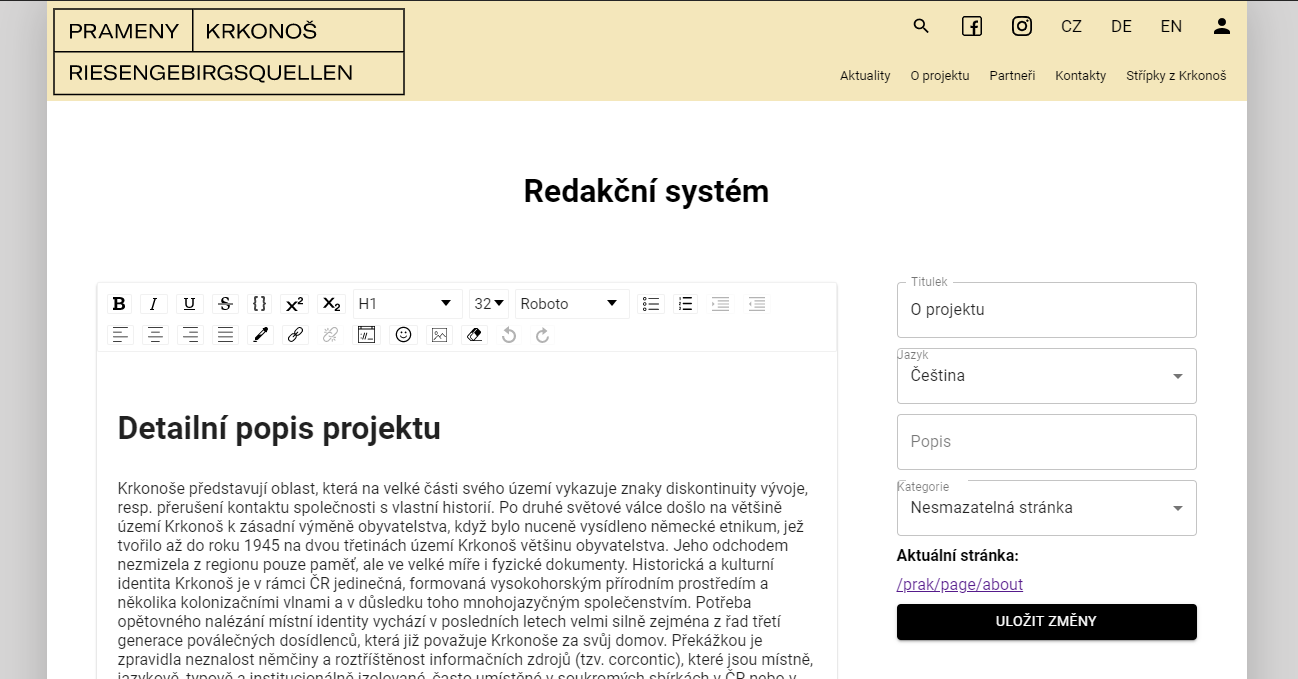
\includegraphics[width=.8\textwidth]{img/cmsScene.png}
\end{center}

\subsubsection{Domovská stránka}
Výchozí stránka na kterou se uživatel dostane, pokud nezadá přesnější cestu v url, je domovská stránka.\\
Na této stránce najde dynamické zobrazování novinek a krátkého popisu v hormím panelu a stránku
s názvem \uv{homepage}, což je obyčejná stránka editovatelná v redakčním systému a dovoluje tedy
redaktorům měnit i domovskou stránku.
\begin{center}
	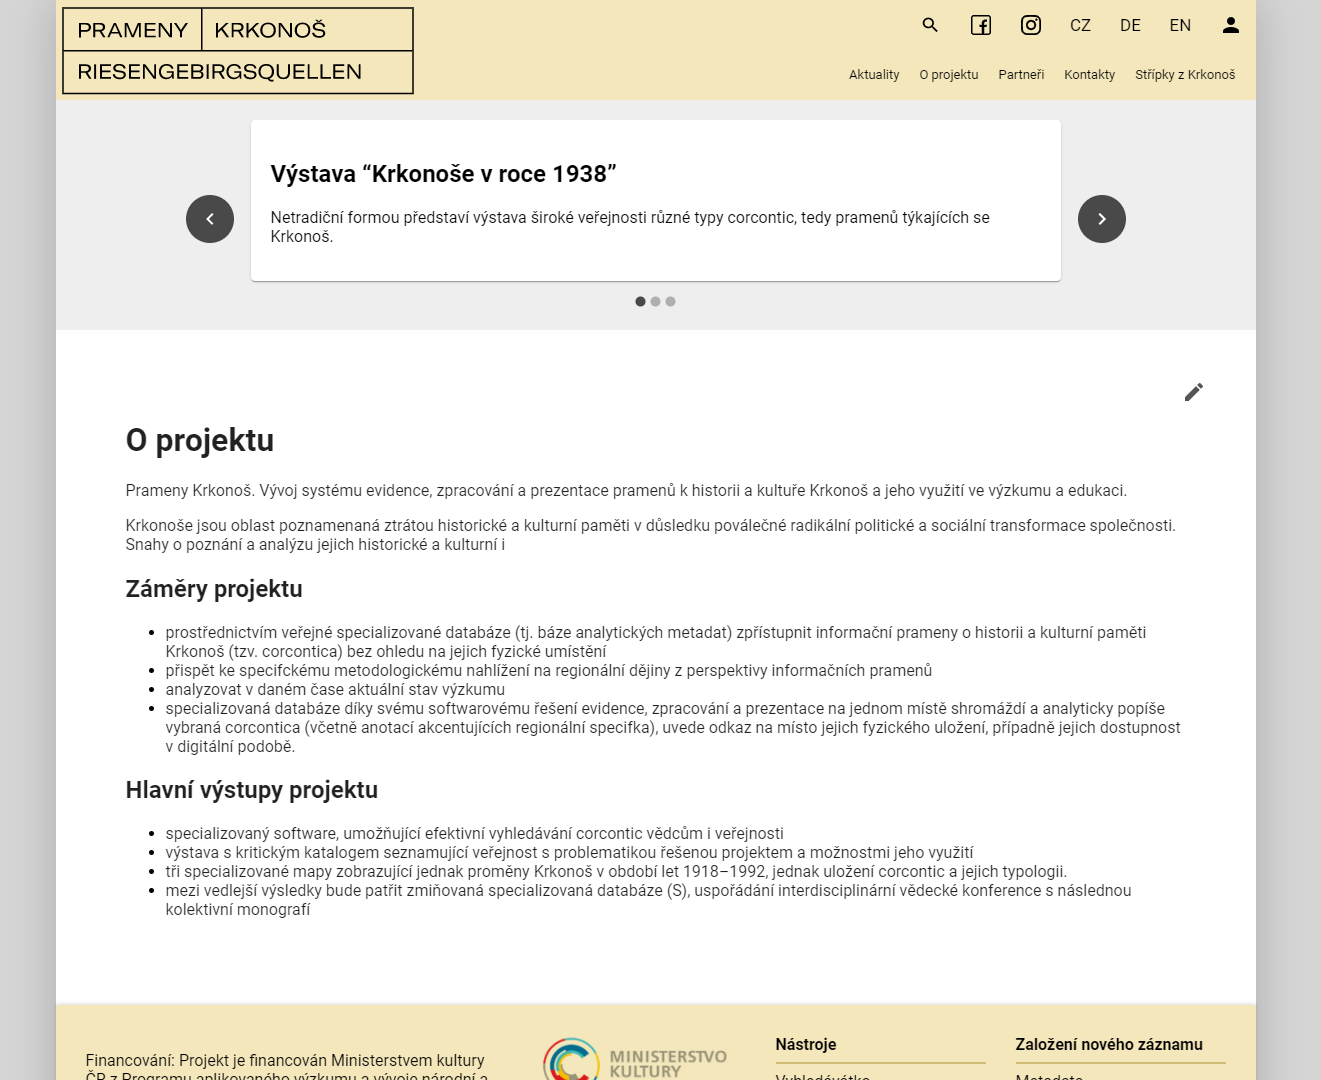
\includegraphics[width=.8\linewidth]{img/homeScene.png}
\end{center}

\subsubsection{Zobrazeni stránky}
Každá stránka vytvořená v redakčním systému je přístupná na adrese \uv{.../prak/page/\#jmenoStranky}.
Zde si ji můžou uživatelé zobrazit. Pokud má uživatel i právo pro redakční systém,
tak se mu v pravém horním rohu zobrazí ikonka pro editaci, díky které se snadno dostane do
redakčního systému pro danou stránku.
\begin{center}
	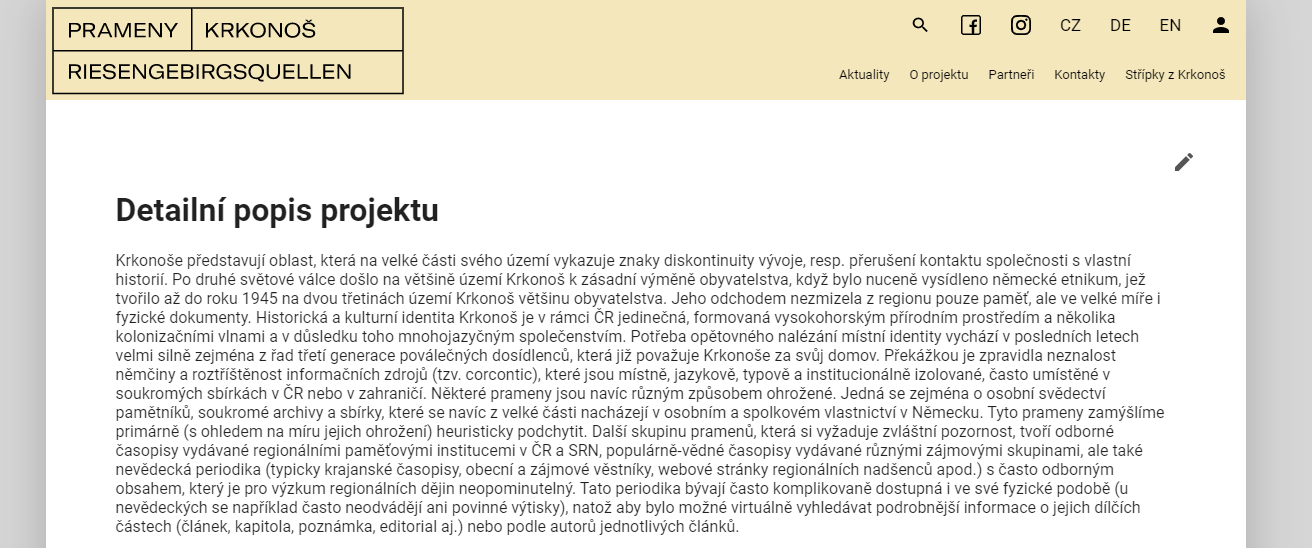
\includegraphics[width=.8\textwidth]{img/pageScene.png}
\end{center}

\subsubsection{Přihlašování}
Pokud uživatel klikne na ikonku postavičky vpravo v hlavičce, nebo se pokusí dostat
na stránku, ke které nemá oprávnění, je přesměrován do přihlašovacího prostředí.
Pokud se poté přihlásí, nebo již přihlášen byl zobrazí se mu podrobnosti o jeho účtu,
včetně dostupných oprávnění.\\
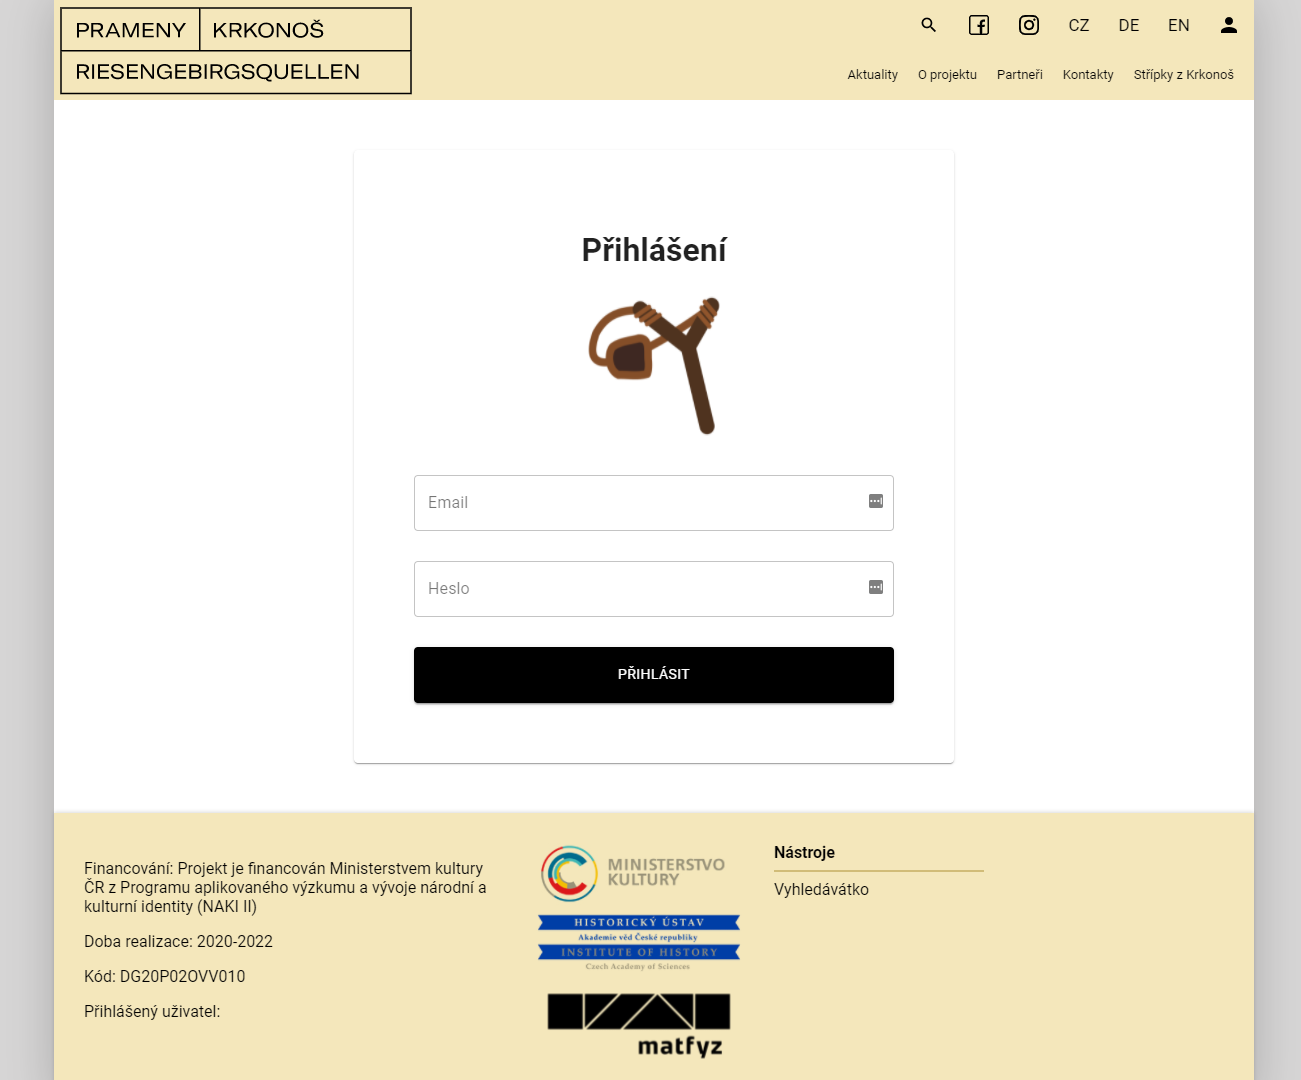
\includegraphics[width=.5\textwidth]{img/loginSceneB.png}
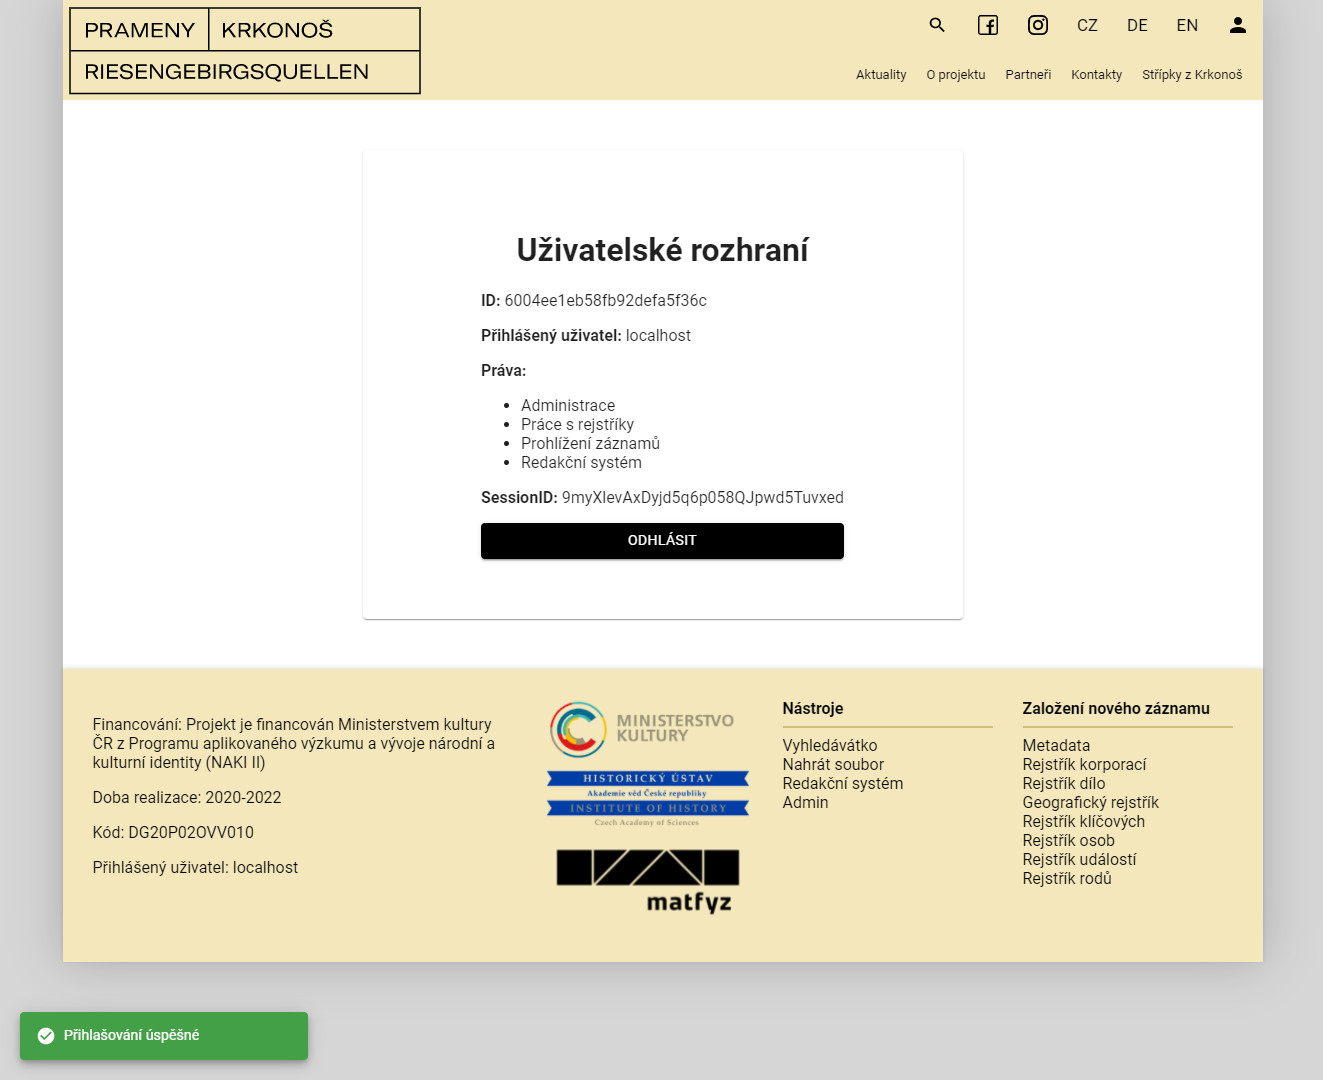
\includegraphics[width=.5\textwidth]{img/loginSceneA.png}

\subsubsection{Kontaktní formulář}
Pro zpětnou vazbu, či otázky k projektu, můžou návštěvníci využít kontaktní formulář.
\begin{center}
	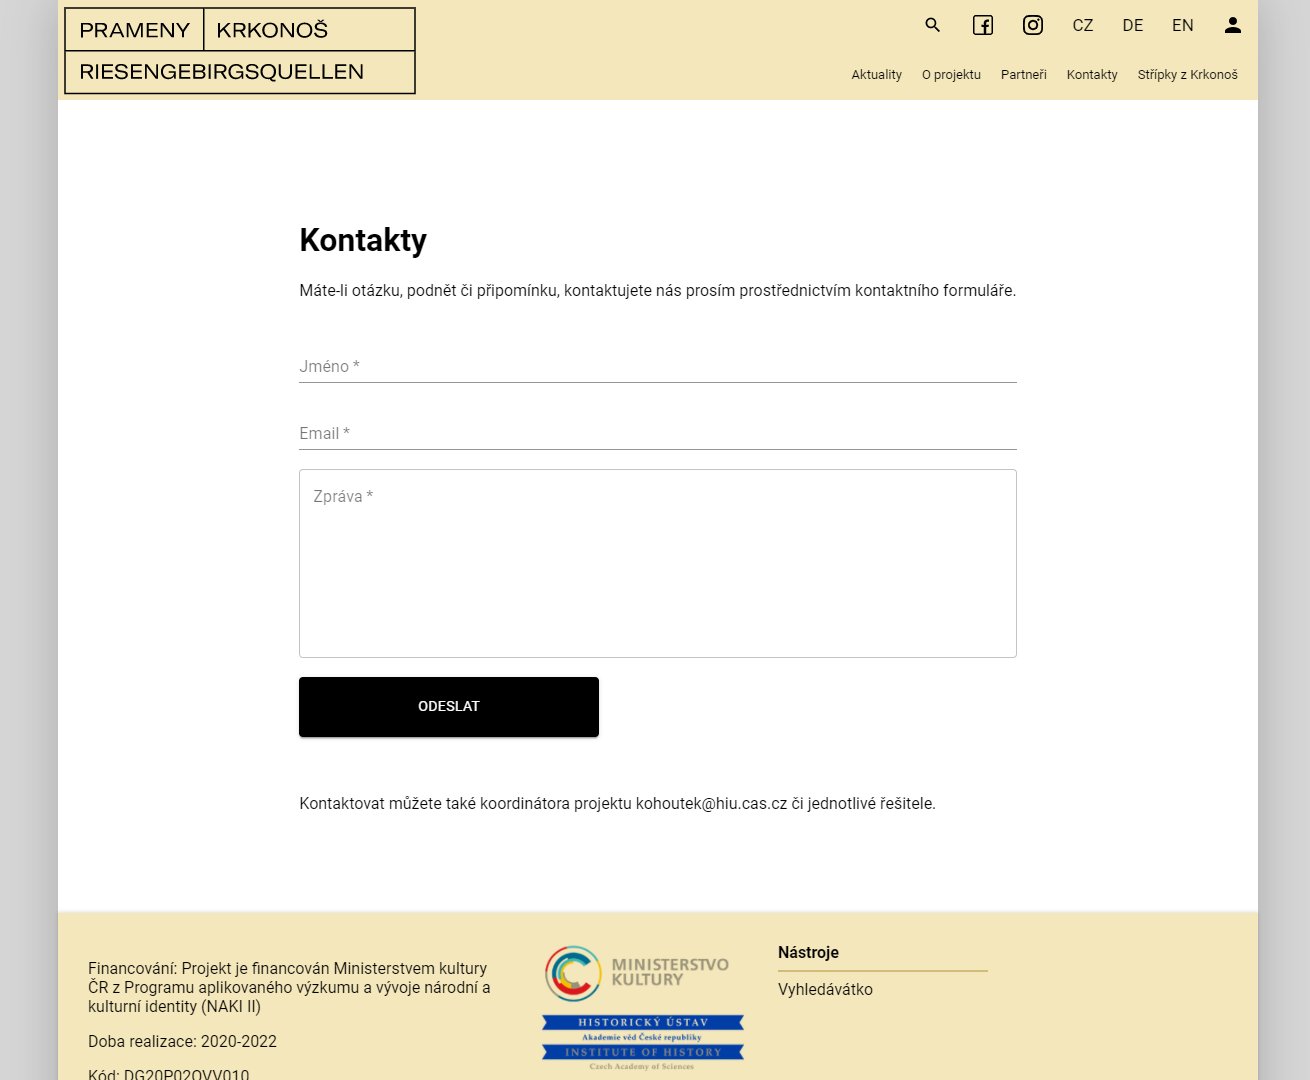
\includegraphics[width=.8\textwidth]{img/contactScene.png}
\end{center}

\subsubsection{Vyhledávátko}
Pomocí ikonky lupy v hlavičce se dostaneme do vyhledávacího prostředí.\\
Po výběru kde chceme hledat se nám načtou políčka k vyplnění. Uživatel do nich může zadat
libovolný výraz a to s podporou regexp syntaxe. Ihned při vyplňování se načítá až 5
prozatím nejvhodnějších výskytů hledání. Při kliknutí na tlačítko \uv{vyhledat} se provede
vyhledání všech odpovídajíchích záznamů.\\
Nalezené záznamy se objevují v tabulce pod vyhledávacím polem.
Tabulka dokáže záznamy třídit po kliknutí na hlavičku příslušného sloupce.
Po kliknutí na záznam se otevře editační prostředí pro vybraný záznam.
\begin{center}
	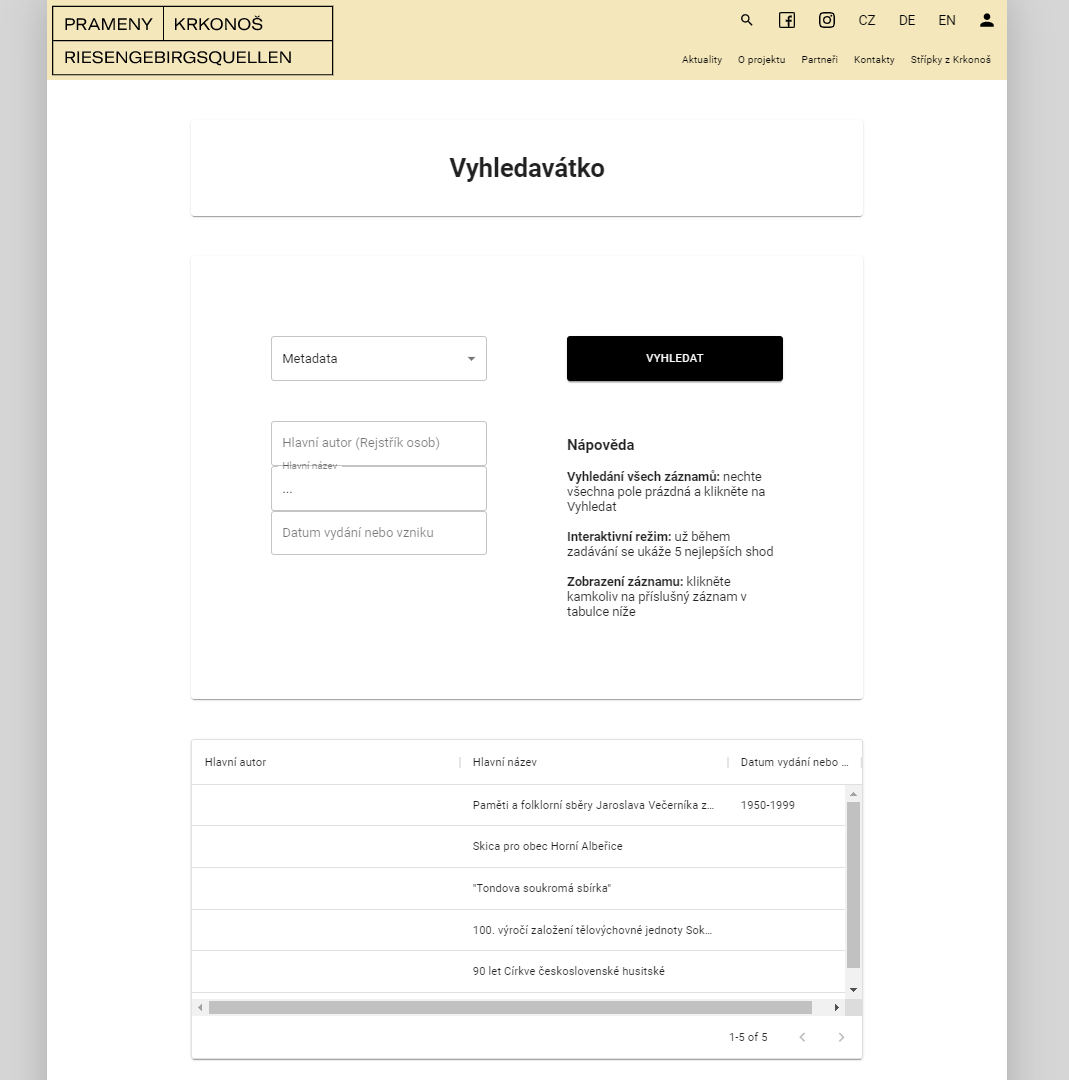
\includegraphics[width=.8\textwidth]{img/searchScene.png}
\end{center}

\subsubsection{Zobrazovávátko}
Záznam uložený v databázi si je možné zobrazit přes toto rozhranní poté co
se k němu dostanete přes vyhledávací rozhranní, nebo pomocí unikátního
url linku, který se po vytvoření záznamu již nemění.\\
Po načtení se uživateli zobrazí záznam, tak jak je uložen v databázi, případně
s přeloženými názvy, pokud to má pomocí spodního přepínátka povolené.
Dole též najde dvě tlačítka pro smazání záznamu a editaci, jež uživatele
přesune do editačního rozhranní s aktuálním záznamem (samozřejmě jen pokud 
má dostatečná oprávnění).
\begin{center}
	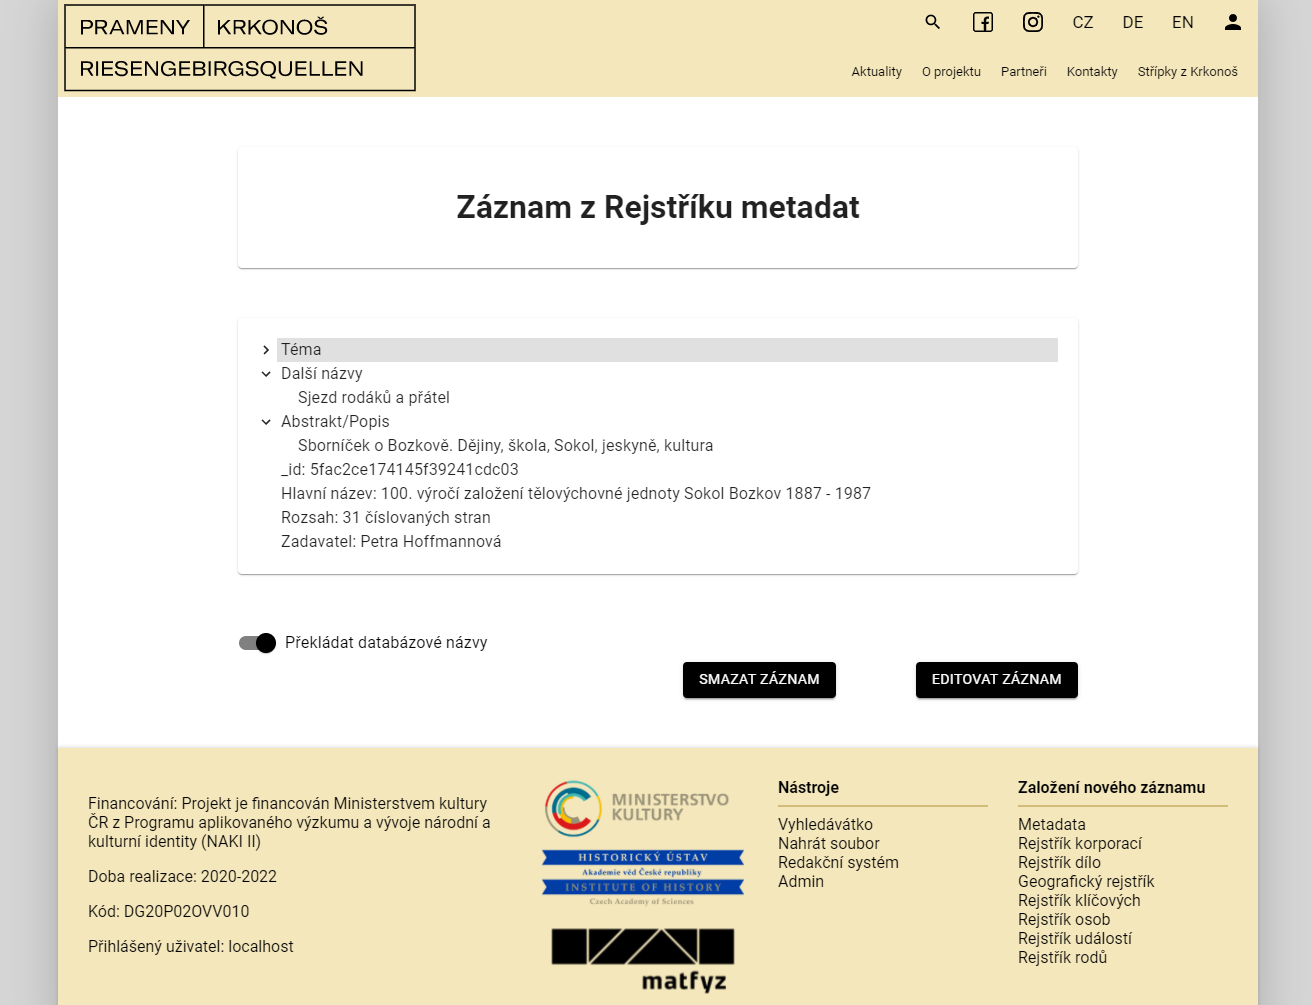
\includegraphics[width=.8\textwidth]{img/showScene.png}
\end{center}

\subsubsection{Upravovátko}
V tomto prostředí je možné záznam upravovat a jedná se o nejkomplikovanější scénu ze všech.\\
Každý typ záznamu a každý podtyp metadatové struktury má vlastní příslušná datová pole.
Ty které umožňují mít více hodnot mají pravo u sebe tlačítka plus a mínus,
jehož velikost určuje velikost bloku, jež je jedním celkem. Plusové tlačítko přidává
další datové pole, zatímco mínus datové pole vyprázdní a poté odebere z náhledu.\\
Datová pole jsou roztřízena do menších podbloků, které se nechají minimalizovat (bez ztráty dat),
aby uživateli usnadnily orientaci. Po minimalizaci resp. maximalizaci bloku může dojít k převážení
sloupců a některé bloky tak mohou střídat levý a pravý sloupec, tak aby celková stránka byla co nejkratší
a prázdného místa byla co nejméně.\\
Některé záznamy mají možnost nahrát přílohu, ta se aktivuje po kliknutí na tlačítko uploadu, s ikonkou šipky
směrem nahoru. Nahraný soubor se ihned přenáší na server a do příslušného pole automaticky 
zaznmená aktuální url nahrávaného souboru.\\
Po kliknutí nahrát se buď objeví červené vyskakovací okno s chybou, proč záznam nelze uložit
(většinou zapříčiněný zadáním unikátního názvu, jež již je v databázi uložen).
Nebo se stránka znovu přepne do zobrazovátka a vyskočí zelené potvrzovací okénko.
\begin{center}
	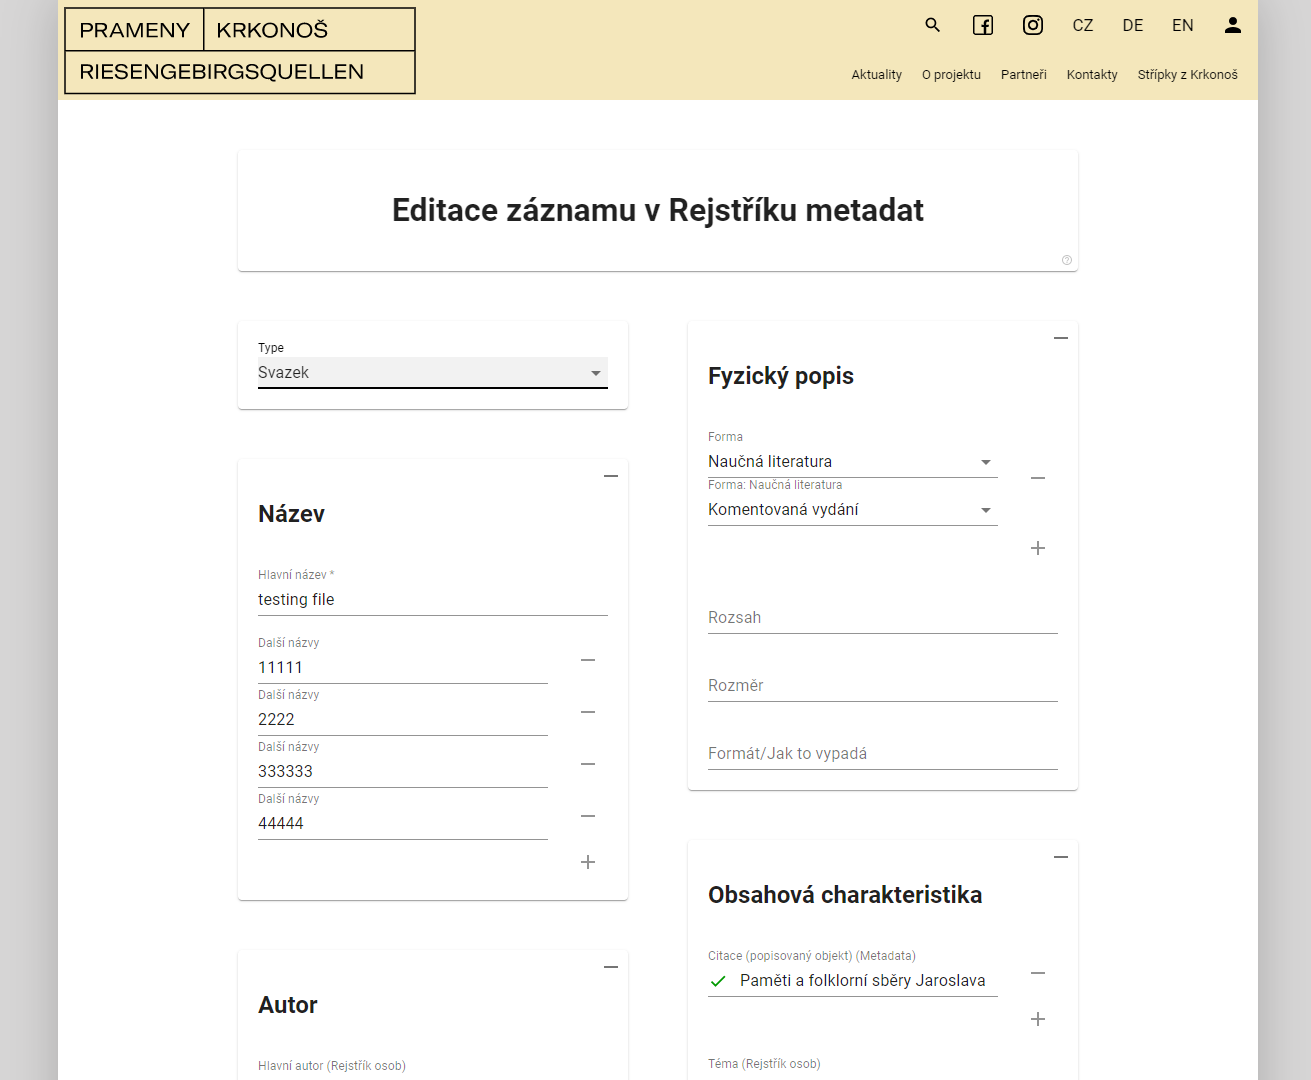
\includegraphics[width=.8\textwidth]{img/editScene.png}
\end{center}


\subsection{Komponenty}
Komponenty jsou vlastně zapouzdřené třídy, které se dají použít vícekrát.
Každá komponenta je chodná pro React systém a většinou je psaná bez tkz. hooků.

\subsubsection{ComboBox}
\begin{wrapfigure}{r}{0.4\textwidth}
	\centering
	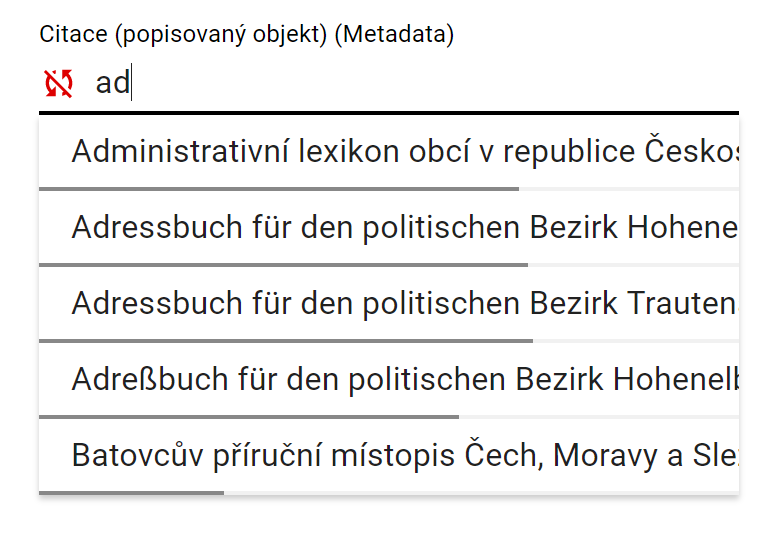
\includegraphics[width=\linewidth]{img/ComboBox.png}
\end{wrapfigure}
ComboBox je textové pole, které při vyplňování realtime vyhledává v databázi vyhovující shody,
které zobrazuje ve formě nabídky pod tímto textovým vstupem. Po kliknutí na nabízenou položku se
do pole vyplní hodnota a na pozadí se do pole uloží ID záznamu (to se poté odesílá na server).
Dokud uživatel některý ze záznamů nevybere, pole není v konzistentním stavu a nemá možnost se
odeslat na server, což značí ikonka

\includegraphics[height=\fontcharht\font`\B]{img/notSynced.png},
v případě že pole má přiřazené id záznamu a zobrazuje název, rozsvítí se ikonka

\includegraphics[height=\fontcharht\font`\B]{img/synced.png},
která značí že data z tohoto pole se při uložení správně odešlou na server.
Popisky často bývají dlouhé a proto je zde i miniaturní posuvník, se kterým se
dá pohodlně pracovat pomocí najetí myši na políčko, přidržení klávesy \textit{Shift} a
točením kolečka na myši.

\subsubsection{Zápatí}
Jako každá správná stránka i v tomto projektu najdeme zápatí, jež obsahuje povinné údaje o projektu a
rychlé odkazy.\\
Jelikož se jedná o projekt Evropské unie, nalezneme zde povinné údaje, kód projektu a
loga sponzora, zadavatelů a vývojářů.
Níže je ukazatel aktuálně příhlášeného uživatele.
V pravé části jsou pak rychlé odkazy, které se zobrazují v závislosti na právech přihlášeného uživatele.
Nepřihlášený uživatel tudíž v této části uvidí pouze jedno menu \uv{Nástroje} s jedinou
položkou \uv{Vyhledávátko} a po přihlášení se viz obázek menu rozroste o dalsí rychlé odkazy.
\begin{center}
	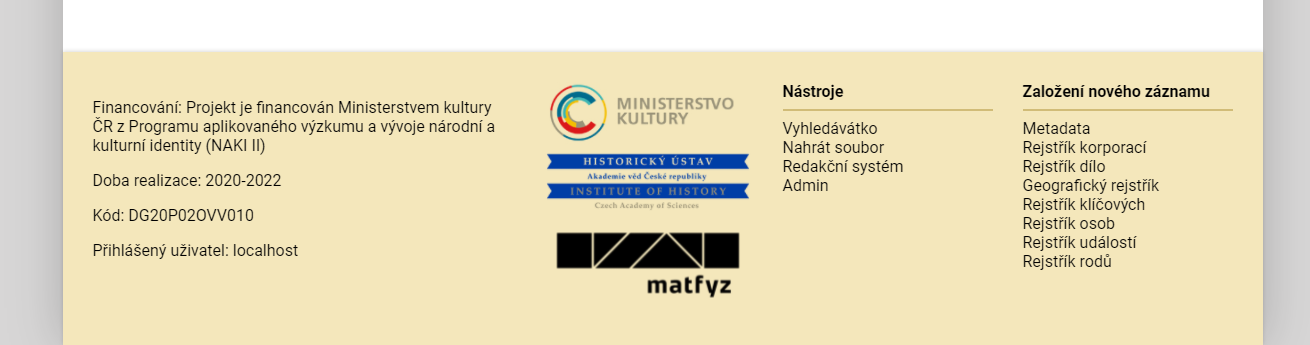
\includegraphics[width=.8\textwidth]{img/zapati.png}
\end{center}

\subsubsection{Navigační menu}
V navigačním menu nalezneme rychlé odkazy na vyhledávátko (tlačítko s ikonkou lupy),
facebook a instagram projektu Prameny Krkonoš a přihlašovací stránku. Tlačítka pro
přepínání mezi třemi jazyky. Níže pak hlavní stránky a seznamové stránky (např. stránka s aktualitami).
\begin{center}
	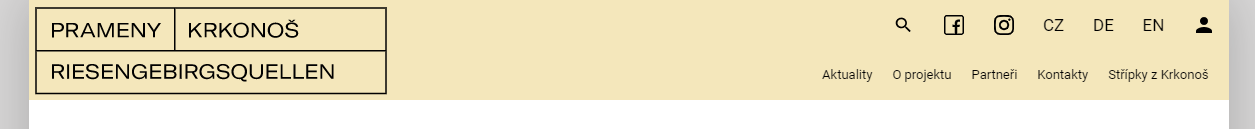
\includegraphics[width=.8\textwidth]{img/navigationBar.png}
\end{center}

\subsubsection{Textové pole s validací}
\begin{wrapfigure}{r}{0.4\textwidth}
	\centering
	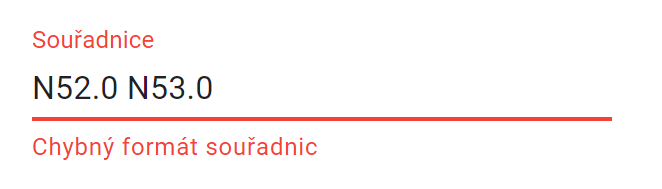
\includegraphics[width=\linewidth]{img/validationField.png}
\end{wrapfigure}
Jako kontrola, že uživatel zadává data ve srozumitelném formátu (tak aby je dokázal pochopit další
uživatel nebo aby je databáze správně interpretovala) jsou data kontrolována na straně klienta.
V případě že data požadovaný formát nemají, pod políčkem se zobrazí varovný nápis a
záznam nepůjde uložit, dokud všechna pole nejsou ve správném formátu.

\subsubsection{Pole pro nahrávání souborů}
\begin{wrapfigure}{r}{0.4\textwidth}
	\centering
	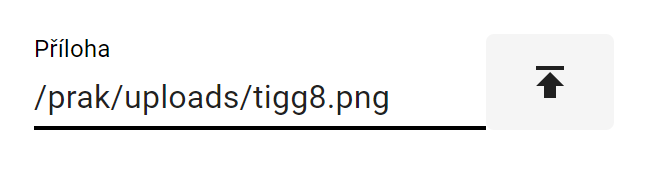
\includegraphics[width=\linewidth]{img/uploadField.png}
\end{wrapfigure}
Některé záznamy a stránky potřebují obsahovat přílohu ve formátu obrázku nebo dokumnetu.\\
Tyto soubory lze nahrát na server a do databáze uložit pouze odkaz na jejich umístění,
protože databáze není stavěná na uchovávání obrázků a podobných relativně velkých souborů.

\subsubsection{Indexy}
Hlavní částí editačního rozhraní jsou indexové objekty, které určují, která pole
se mají zobrazit při různých typech záznamů. Pro každý typ je zde JSON soubor, ve kterém
je seznam polí a informace o nich. Mezi tyto informace patří především popisek, struktura jak
data odeslat do databáze, nápověda přístupná pomocí malého otazníčku a nepoviná pole jako
požadavek na nenulovou hodnotu, nebo regexpový výraz pro kontrolu formátu dat.

\subsection{Moduly}
Funkcionalita, která není až tak často používána, se do hlavního souboru aplikace
nepřidává a tudíž čistý frontend žádné moduly nepodporuje. Moduly jsou výhradně načítány
ze serveru a neobsahují hlavní frontend.

\section{Lokalizace}
Překlad stránky do různých jazyků je řešen pomocí knihovny i18n, která je velmi efektivní a
zároveň poskytuje snadný způsob jak texty překladu přidávat a editovat. 
Překlady navíc jsou rozloženy do více souborů a úrovní, takže se překlad velmi dobře
škáluje i na větší projekty.\\
Výsledkem jsou lokalizační soubory ve formátu JSON, které frontend aplikuje na požadovaných
místech. Pokud ovšem překlad chybí použije se nejbližší možná interpretace, podobný jazyk, nebo
zdrojová adresa překladu a vývojáři ukáže zprávu o chybějícím překladu.
